\documentclass[11pt,twoside,a4paper]{article}

% ─────────────────────────────────────────────────────────────
%  ORACLE user-manual preamble: shared packages, styling, macros
%  (DENIS's, carried over)
% ─────────────────────────────────────────────────────────────

% Encoding & fonts
\usepackage[utf8]{inputenc}
\usepackage[T1]{fontenc}
\usepackage{lmodern}
\usepackage{textcomp}

% Page layout
\usepackage[a4paper,top=2.5cm,bottom=2.5cm,left=2.5cm,right=2.5cm,
            headheight=14pt]{geometry}
\usepackage{microtype}
\emergencystretch=3em                          % long paths break cleanly
\raggedbottom

% Headers / footers
\usepackage{fancyhdr}
\pagestyle{fancy}
\fancyhf{}
\fancyhead[LE,RO]{\thepage}
\fancyhead[LO]{\textit{\nouppercase{\rightmark}}}
\fancyhead[RE]{\textit{ORACLE User Manual}}
\renewcommand{\headrulewidth}{0.4pt}

% Math, units
\usepackage{amsmath}
\usepackage{amssymb}

% Lists
\usepackage{enumitem}
\setlist{itemsep=2pt, parsep=0pt}

% Tables
\usepackage{booktabs}
\usepackage{array}
\usepackage{tabularx}
\newcolumntype{L}{>{\raggedright\arraybackslash}X}

% Graphics
\usepackage{graphicx}
\graphicspath{{figs/}}
\usepackage{caption}
\usepackage[section]{placeins}                 % figures stay in their section
\captionsetup{font=small, labelfont=bf, margin=10pt}

% Code listings
\usepackage{xcolor}
\definecolor{codebg}{HTML}{F5F5F5}
\usepackage{listings}
\lstset{
    basicstyle=\ttfamily\small,
    backgroundcolor=\color{codebg},
    frame=single,
    framesep=4pt,
    rulecolor=\color{black!20},
    breaklines=true,
    columns=fullflexible,
    showstringspaces=false,
    aboveskip=8pt,
    belowskip=8pt,
}

% Hyperlinks
\usepackage[colorlinks=true,
            urlcolor=blue!60!black,
            linkcolor=black,
            citecolor=blue!60!black]{hyperref}

% ─── ORACLE-specific macros ──────────────────────────────────
\newcommand{\oracle}{\textsc{ORACLE}}
\newcommand{\denis}{\textsc{DENIS}}
\newcommand{\app}[1]{\textsf{\textbf{#1}}}     % UI element / button name
\newcommand{\menu}[1]{\textsf{#1}}             % menu path, e.g. \menu{File > Open run...}
\newcommand{\code}[1]{\texttt{\small #1}}      % inline code / paths / keys
\newcommand{\us}{\,$\mu$s}                     % microseconds


\title{%
    {\Huge\bfseries ORACLE}\\[2pt]
    {\large User Manual}\\[6pt]
    {\normalsize\itshape Online Readout \& Acquisition for Collinear Laser spectroscopy
     Experiments}\\[10pt]
    {\normalsize Version 0.6.0}
}
\author{Ethan Barnes \\ \texttt{ethan.barnes@postgrad.manchester.ac.uk}}
\date{\today}

\begin{document}

\maketitle
\thispagestyle{empty}
\clearpage

\tableofcontents
\clearpage

\section{Introduction}
\label{sec:introduction}

\oracle{} is the data acquisition for collinear laser spectroscopy (CLS) at IGISOL. It steps
the platform voltage through a scan, records every ion the time tagger sees against the
voltage it was taken at, and calibrates the voltage axis before every run. It keeps the
collinear DAQ's layout, file format and functions, brings in the bench calibration tool
cls-cal~\cite{clscal}, and is built so that the faults found in the old DAQ cannot happen
rather than being caught afterwards (Appendix~\ref{sec:design}). Runs are read by
cls\_tools~\cite{clstools} and fitted in \denis{}~\cite{denis}, both unchanged.

The window has five tabs above the quick-tune controls and the experiment information:

\begin{description}
    \item[\app{Scan controls}.] Scan and buncher parameters, run control, the scan queue,
        the ELOG panel and the live plots (Section~\ref{sec:scan}).
    \item[\app{Scan Calibration}.] A stand-alone calibration and the gate's verdict on it;
        every scan's own calibration is shown here too (Section~\ref{sec:calibration}).
    \item[\app{Hardware Calibration}.] The bench tool's measurements of the rack itself:
        settle time, linearity, the cooler, the bench table and the health check
        (Section~\ref{sec:hardware}).
    \item[\app{Scan Performance}.] How the rack's behaviour during a run shaped its
        spectrum, check by check, with the run's systematic inputs
        (Section~\ref{sec:performance}).
    \item[\app{Time graphs}.] Counts against time, to watch the beam.
\end{description}

\paragraph{Principles.}
Every calibration point is written, confirmed and only then read, so the voltage axis
cannot slip. Nothing is cut: what deserves a look is flagged, and the operator decides in
\denis{}. Every input survives a crash, and a run can be reopened exactly as it was taken.

\paragraph{Status.}
\oracle{} runs end to end on its simulated rack, which imitates the rack the bench tool
measured in October 2026. It has not yet driven the beamline: its drivers follow code that
has run on the rack but are tested against stand-ins for the vendor libraries.

\paragraph{Scope.}
This is a user manual. The code (\code{cls\_acquisition/}, \code{gui/}) documents itself
for developers; the README describes the test suite.

\section{Installation}
\label{sec:installation}

\oracle{} runs on Windows and macOS (and Linux, simulated only). The installers use
\code{uv}, which brings its own Python, so none need be installed.

\begin{lstlisting}[language=bash]
git clone https://github.com/EthanBarnes54/ORACLE.git
cd ORACLE
install.bat full       # Windows
./install.sh full      # macOS / Linux
\end{lstlisting}

\begin{center}
\begin{tabularx}{\textwidth}{@{}lL@{}}
\toprule
Option & Does \\
\midrule
\code{full}     & uv, the dependencies and a desktop shortcut (on macOS an \code{ORACLE.app}
                  in \code{\textasciitilde/Applications}, linked from the Desktop) \\
\code{rack}     & as \code{full}, plus the instrument libraries (pyvisa, pyepics, py-elog,
                  spinapi, mcculw): for the beamline PC \\
\code{uv}       & uv alone \\
\code{shortcut} & the shortcut alone \\
\bottomrule
\end{tabularx}
\end{center}

With no option the installer offers a menu. Launch from the shortcut, or with
\code{uv run python gui.py}. To update, \code{git pull} then \code{uv sync}.

\paragraph{Simulated or hardware.}
\oracle{} starts on the simulated rack: the status bar says \app{Simulated rack}, runs go
to \code{data/simulated}, and nothing is posted to the ELOG. On the beamline PC, install
with \code{rack} and set \code{rack: hardware} in \code{settings/settings.yaml}
(Section~\ref{sec:settings}).

\paragraph{The time tagger's wrapper.}
The collinear DAQ's compiled TimeTagger4 wrapper has four faults (Appendix~\ref{sec:design}).
Build the corrected one on the rack PC, with Visual Studio's C++ build tools and the
cronologic driver installed:

\begin{lstlisting}
cd cls_acquisition\hardware\timetagger4_wrapper
uv run --with pybind11 --with setuptools python build_wrapper.py
\end{lstlisting}

\noindent then set \code{instruments: tagger\_driver} to that folder. Until it is built,
the status bar carries a rack warning naming the inputs affected.

\paragraph{Where things are kept.}
\code{settings/} holds \code{settings.yaml} (yours), \code{inputs.yaml} (the window's last
inputs) and \code{rack.yaml} (the last rack of each kind); \code{data/} the runs and
records (Section~\ref{sec:data}); \code{logs/} a session log per launch, the newest 20 kept.
\menu{File > Open data folder} and \menu{Open log folder} open them.

\section{Quick start}
\label{sec:quickstart}

\subsection{A first scan, on the simulated rack}

\begin{enumerate}
    \item Launch \oracle{}. On \app{Scan controls}, tick the first range and set
        \app{From (V)} 15 and \app{To (V)} 85, \app{Stepsize (V)} 1, \app{Bunches per
        channel} 25 and \app{Scan type} Sawtooth.
    \item Press \app{Start scan}. \oracle{} calibrates the scan's own setpoints, puts the
        calibration through the gate, writes the run's header and starts. The plots fill
        as hits arrive (Figure~\ref{fig:scan}); the simulated beam has lines at 32, 47 and
        71\,V.
    \item Press \app{Stop after scan} to end at the end of the scan in progress, or
        \app{Stop now!} to end within a bunch.
    \item The run is analysed as it closes: \app{Scan Performance} gives its verdict, and
        \app{Scan Calibration} its calibration.
    \item \menu{File > Open run...} (Ctrl+O, Cmd+O on macOS) brings any run back as it was
        taken.
\end{enumerate}

\begin{figure}[ht]
    \centering
    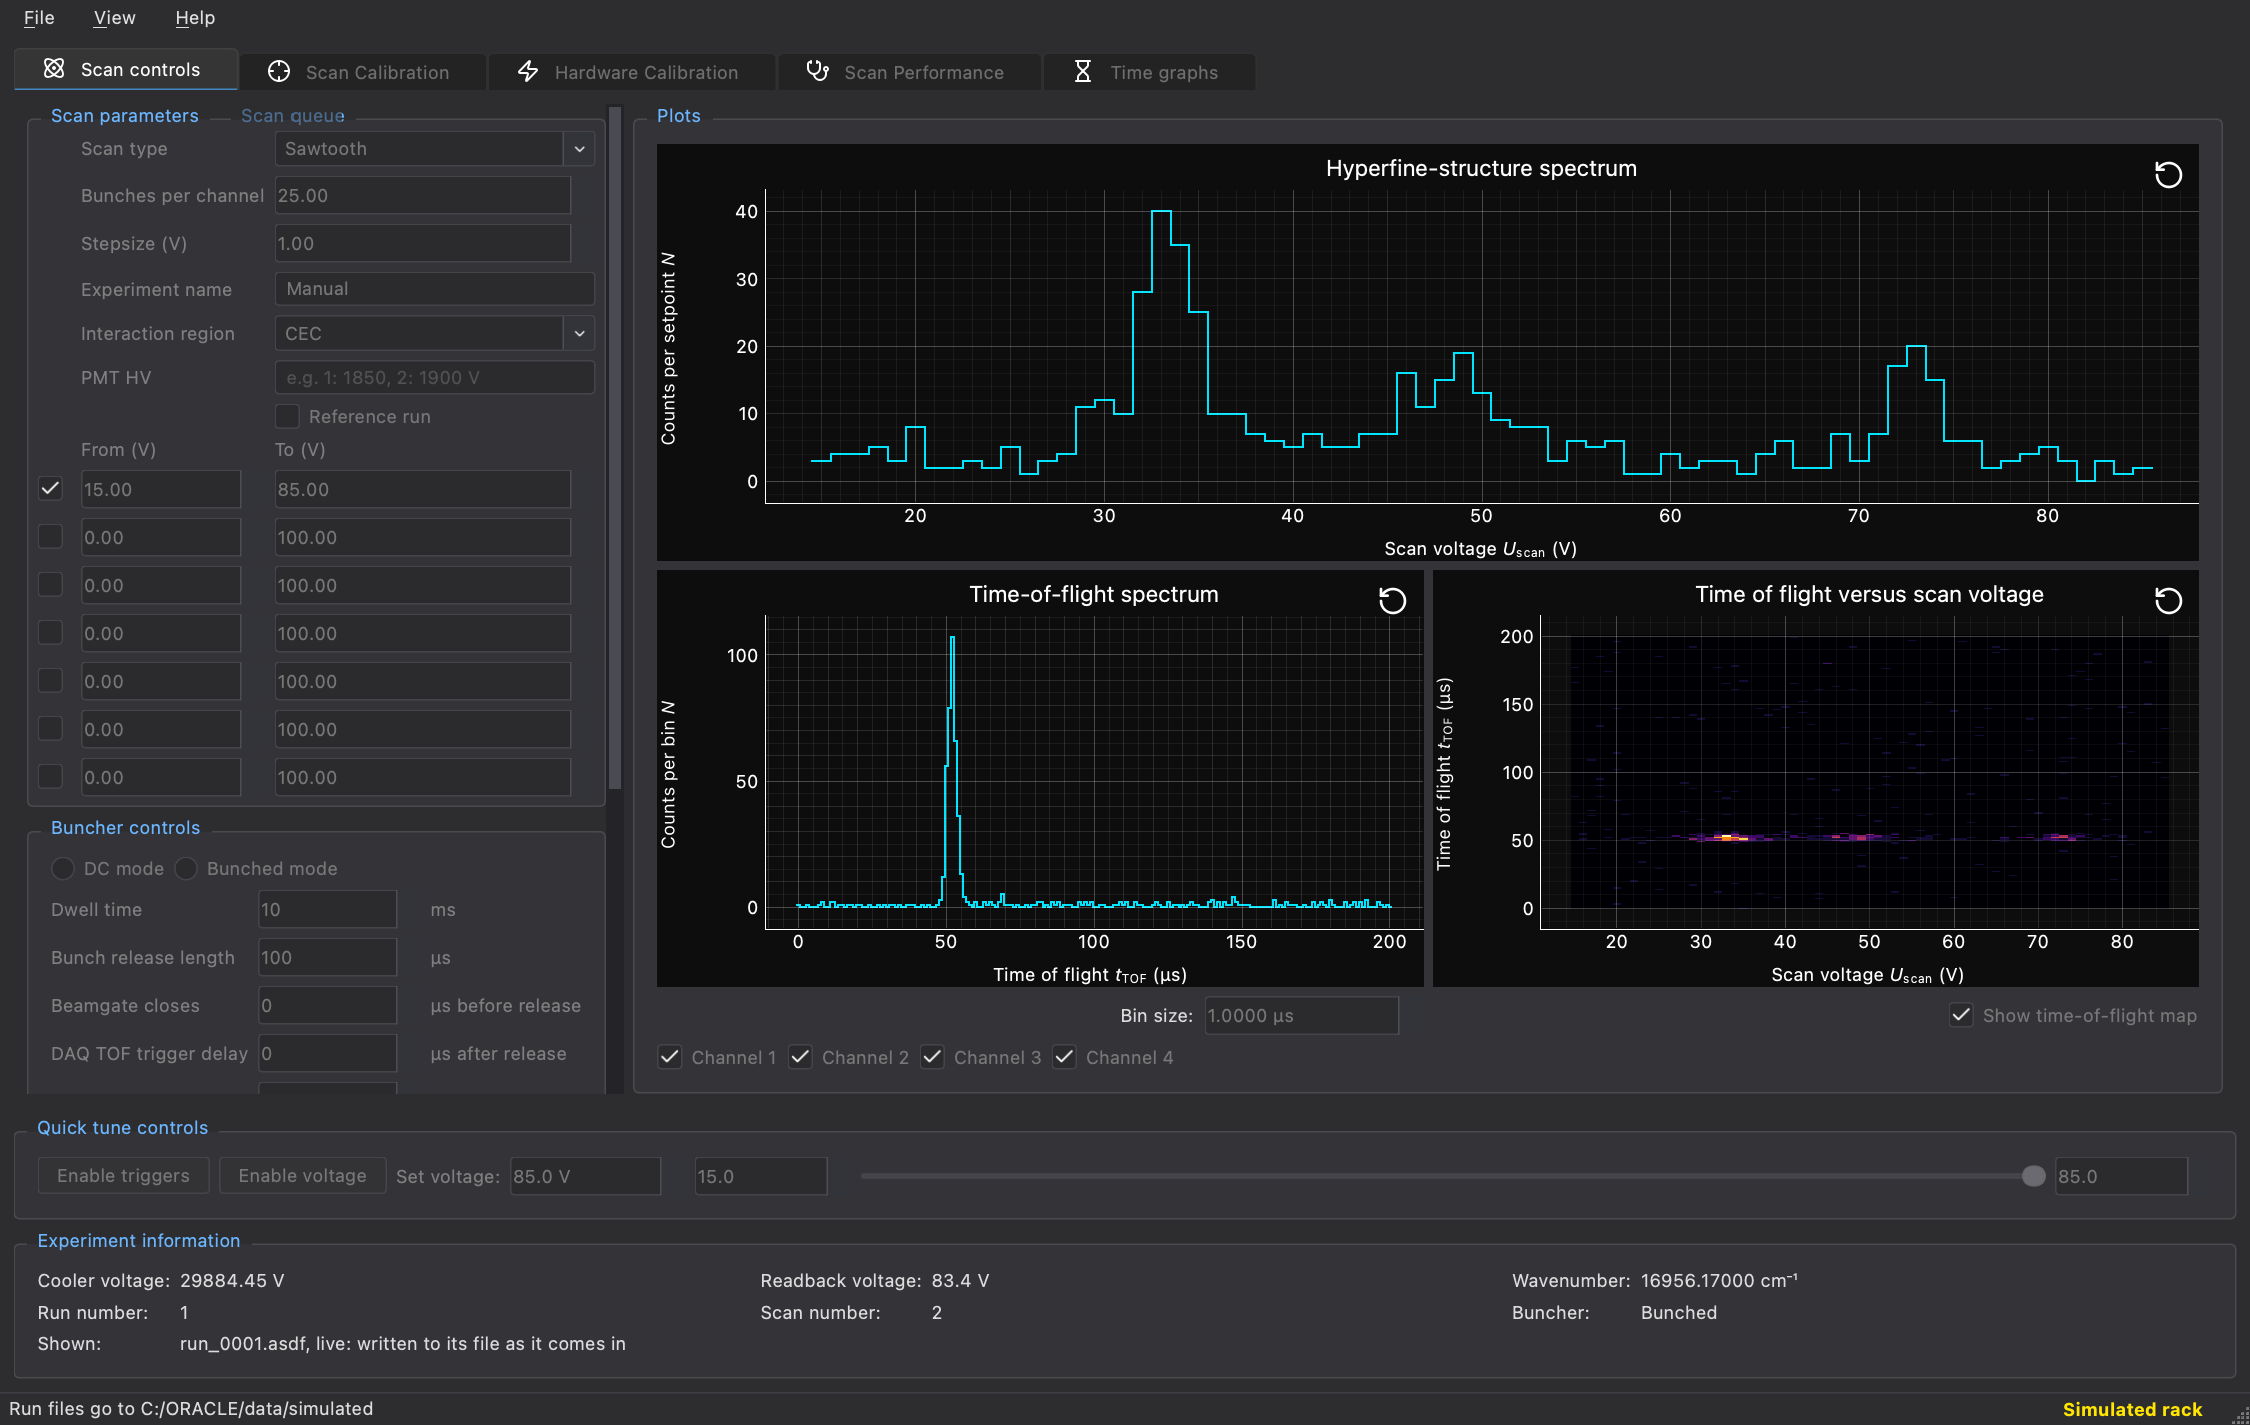
\includegraphics[width=\textwidth]{fig_scan_tab}
    \caption{The \app{Scan controls} tab during a simulated scan: parameters on the left,
        the hyperfine-structure spectrum, time-of-flight spectrum and map on the right,
        quick tune and the experiment information below.}
    \label{fig:scan}
\end{figure}

\subsection{A shift on the beamline}

\begin{enumerate}
    \item Read the status bar. A rack warning (a fault \oracle{} cannot mend, or hardware
        changed since the last session) is named there, its sentence in the tooltip.
    \item Run the \app{Health check} (\app{Hardware Calibration}), with \app{Check the bench
        table first} ticked: the table, the cooler's ripple, each PMT's dark counts, the
        triggers and both meters' trigger sources, set against the last check.
    \item If the hardware changed, measure the settle model (\app{Settle time}) and the
        bench table (\app{Scan table}) again before taking data.
    \item On \app{Scan controls}, set the \app{Experiment name}, the \app{Interaction region}
        and the \app{PMT HV}, and the buncher timing.
    \item Take scans one at a time, or lay them out in the \app{Scan queue} and let it run
        unattended.
    \item Read each run's \app{Scan Performance} verdict, and anything flagged for review,
        before fitting it in \denis{}.
\end{enumerate}

\section{Scan controls}
\label{sec:scan}

\subsection{Scan parameters}

\begin{center}
\begin{tabularx}{\textwidth}{@{}lL@{}}
\toprule
Field & Meaning \\
\midrule
\app{Scan type}          & Sawtooth (repeats up), Triangle (up and back) or Single scan \\
\app{Bunches per channel} & bunches taken at each setpoint; \app{Seconds per channel} in DC mode \\
\app{Stepsize (V)}       & the step between setpoints \\
\app{From (V)}, \app{To (V)} & up to seven ranges, each ticked to be scanned; a point
                           shared by two ranges is visited once \\
\app{Experiment name}    & recorded with every run and in the ELOG \\
\app{Interaction region} & CEC or LCR: the cooler offset differs between them \\
\app{PMT HV}             & the PMTs' high voltage, recorded where EPICS does not give it \\
\app{Reference run}      & marks a run taken to measure the beam's offset from the cooler \\
\bottomrule
\end{tabularx}
\end{center}

Every voltage is held to the platform's limit (by default the Trek 609E-6's $\pm$4\,kV). A
range that is not a whole number of steps ends on its last whole step, never past its stop.

\subsection{Buncher controls}

\app{Bunched mode} takes one bunch per \app{Dwell time}: the buncher is released for
\app{Bunch release length}, and the tagger's window opens \app{DAQ TOF trigger delay} after
the release and stays open from \app{DAQ gate starts} to \app{DAQ gate stops}, inside the
tagger's 8.39\,ms range. \app{DC mode} opens a window every millisecond; its gate stays
settable, since DC hits come through the tagger too. A timing that does not fit its cycle
(a release or delay past its end, a window still open at the next trigger) is refused with
a sentence before anything starts.

\subsection{Starting and stopping}

\app{Start scan} calibrates the scan's own setpoints (Section~\ref{sec:calibration}); only
if the gate passes are the run file written and the scan started. A refused calibration
writes nothing, and its run number is given to the next attempt. \app{Stop after scan}
finishes the scan in progress; \app{Stop now!} ends within a bunch.

At each step the tagger's window is shut, the DAC written, and the window held shut for as
long as the settle model says the jump takes; every step then takes its full count of
bunches at a settled voltage, while the buncher and cooler run on untouched. A tagger that
sees no trigger for three cycles (two seconds at least) is reported on the status bar, and
the scan holds its setpoint until triggers return.

\subsection{Scan queue}

The second page of the parameters box lays scans out ahead, one row and one run file each:
ranges (\code{20:55, 60:80}), step, bunches (seconds in DC), order (Sawtooth or Triangle)
and number of scans; timing, experiment and view are the parameters page's. Each row is
checked as it is typed (a bad cell turns red) and the readout gives each row's setpoints and
time, or its fault, and when the queue ends. \app{Add current} adds the parameters as they
stand, \app{Show} puts a row back on them, rows paste from a spreadsheet, Delete clears
cells.

\app{Automatic} starts each scan as the last ends, so a queue can run overnight;
\app{Manual} asks before each scan after the first. Anything but a clean end (a calibration
refused, a file not written, a scan stopped by hand) stops the queue with the platform at
rest, its row saying why. \app{Stop queue after this scan} lets the running scan finish.
Rows and states survive a crash; a restarted queue takes up at the first scan not done.

\subsection{Plots}

The hyperfine-structure spectrum, the time-of-flight (TOF) spectrum and, with \app{Show
time-of-flight map}, the TOF against scan voltage. Ctrl-drag (Cmd-drag on macOS) on the TOF
spectrum sets the gate, a double-click removes it; the spectrum and map count only hits
inside it. \app{Bin size} and the \app{Channel} boxes choose the TOF binning and the PMTs.
The view is held from Start to the scan's last event and recorded with the run.

Every plot handles alike: drag to pan, right-drag to stretch, the wheel to zoom (over an
axis, that axis alone), Shift-drag to zoom to a box. A plot handled by hand stops following
the data until its \raisebox{-0.1ex}{$\circlearrowleft$} button, a double-click or
\menu{View > Autoscale all plots} (Ctrl+0) returns it. Resting the cursor on a title says
what the plot shows and how it is calculated.

\subsection{ELOG, quick tune and the experiment information}

\app{Send additional text} appends to the open ELOG entry, \app{Start new entry} begins the
next, \app{Send HFS screen} attaches the spectrum. Each scan posts its parameters and
calibration; a simulated rack posts nothing.

\app{Enable triggers} runs the triggers without a scan; \app{Enable voltage} puts
\app{Set voltage} on the platform, set by value or by the slider across its range, starting
from the voltage already there. Spin boxes and the slider take the mouse wheel only once
clicked, so scrolling past them never moves the platform. Below, the cooler and readback
voltages, the wavenumber, run and scan numbers, the buncher mode, and \app{Shown}: the run
every tab is showing, live, saved or opened.

\section{Calibration and the gate}
\label{sec:calibration}

\subsection{Step and confirm}

Every run starts with a calibration of its own setpoints: each commanded platform voltage is
paired with what the line meter reads through the $\times$1000 divider. For each setpoint,
in order,
\begin{enumerate}
    \item the acquisition process writes the DAC and confirms the write;
    \item the meter waits for the point to settle, then takes \emph{one} reading on command;
    \item the reading is kept only if it was taken at least that long after its write;
        otherwise the reading (not the write) is asked for again after the shortfall.
\end{enumerate}
Reading $i$ cannot be asked for before write $i$ is confirmed, so setpoint and reading
cannot slip apart. Each reading integrates whole power line cycles
(\code{calibration: nplc}, 1 by default), which takes out the mains a short reading
catches. Retries are capped at three a point and ten a calibration; any other fault stops
the calibration with a sentence naming it.

\paragraph{Settling.}
SETTLE, 50\,ms, covers the amplifier's measured settling (a 2\,kV jump within 0.5\,V in
20.5\,ms). Where the \app{Settle time} page has measured a settle model, each jump waits
1.25 times its settling, if longer.

\subsection{The gate}

A \textbf{REJECT} writes no file and starts no scan; a \textbf{WARN} goes to the ELOG with
the run. The thresholds are \code{THRESHOLDS} in \code{cls\_acquisition/calibration.py},
and each run records those it was judged by.

\begin{center}
\begin{tabularx}{\textwidth}{@{}lL@{}}
\toprule
Check & Refuses (or warns) when \\
\midrule
length          & there is not one reading per planned setpoint \\
tracking        & the readback does not follow the command ($|r| < 0.90$) \\
span            & the readback's span is more than 10\,\% off the commanded span \\
polarity        & (WARN) the two converters' lines meet 0\,V more than 0.10\,V apart \\
settle          & a kept reading came sooner after its write than its jump takes to settle;
                  (WARN) setpoints were read again \\
held            & the last setpoint, read ten more times held 0.2\,s on, scatters over 0.5\,V,
                  or the calibration's last reading sits more than half a step (or six of
                  their scatter) from it: a lag of $k$ puts it $k$ steps off \\
plan            & the commanded voltages are not the plan, once each, in order \\
dac\_calibration & a measured DAC correction is past its validity; (WARN) one is in force,
                  since the bench table is applied after collection \\
\bottomrule
\end{tabularx}
\end{center}

\subsection{The Scan Calibration tab}

A calibration over any range, without a scan: set \app{From (V)}, \app{To (V)} and
\app{Stepsize (V)} and press \app{Start calibration}. The readback against setpoint, its
deviation and the measured step fill point by point; the gate's verdict and every check
follow (Figure~\ref{fig:calibration}). A scan's own calibration and an opened run's are
shown here too.

\paragraph{Against the bench table.}
With a bench table in force (Section~\ref{sec:table}), every calibration is fitted to it,
$V = a + b\,T$ at each point's DAC code, weighted by the meter's noise and the table's
10\,mV repeatability. The report gives $a$ (the run's 0\,V level), $b - 1$, the residual
against what those account for (WARN at twice that: the table is stale or the hardware
changed), how many points fell between the table's codes, and $a$ and $b$ of the last runs
on the same table. The fit is recorded with the run (\code{TableFit}); the header's
\code{CalSet} and \code{CalReadback} are unchanged.

\begin{figure}[ht]
    \centering
    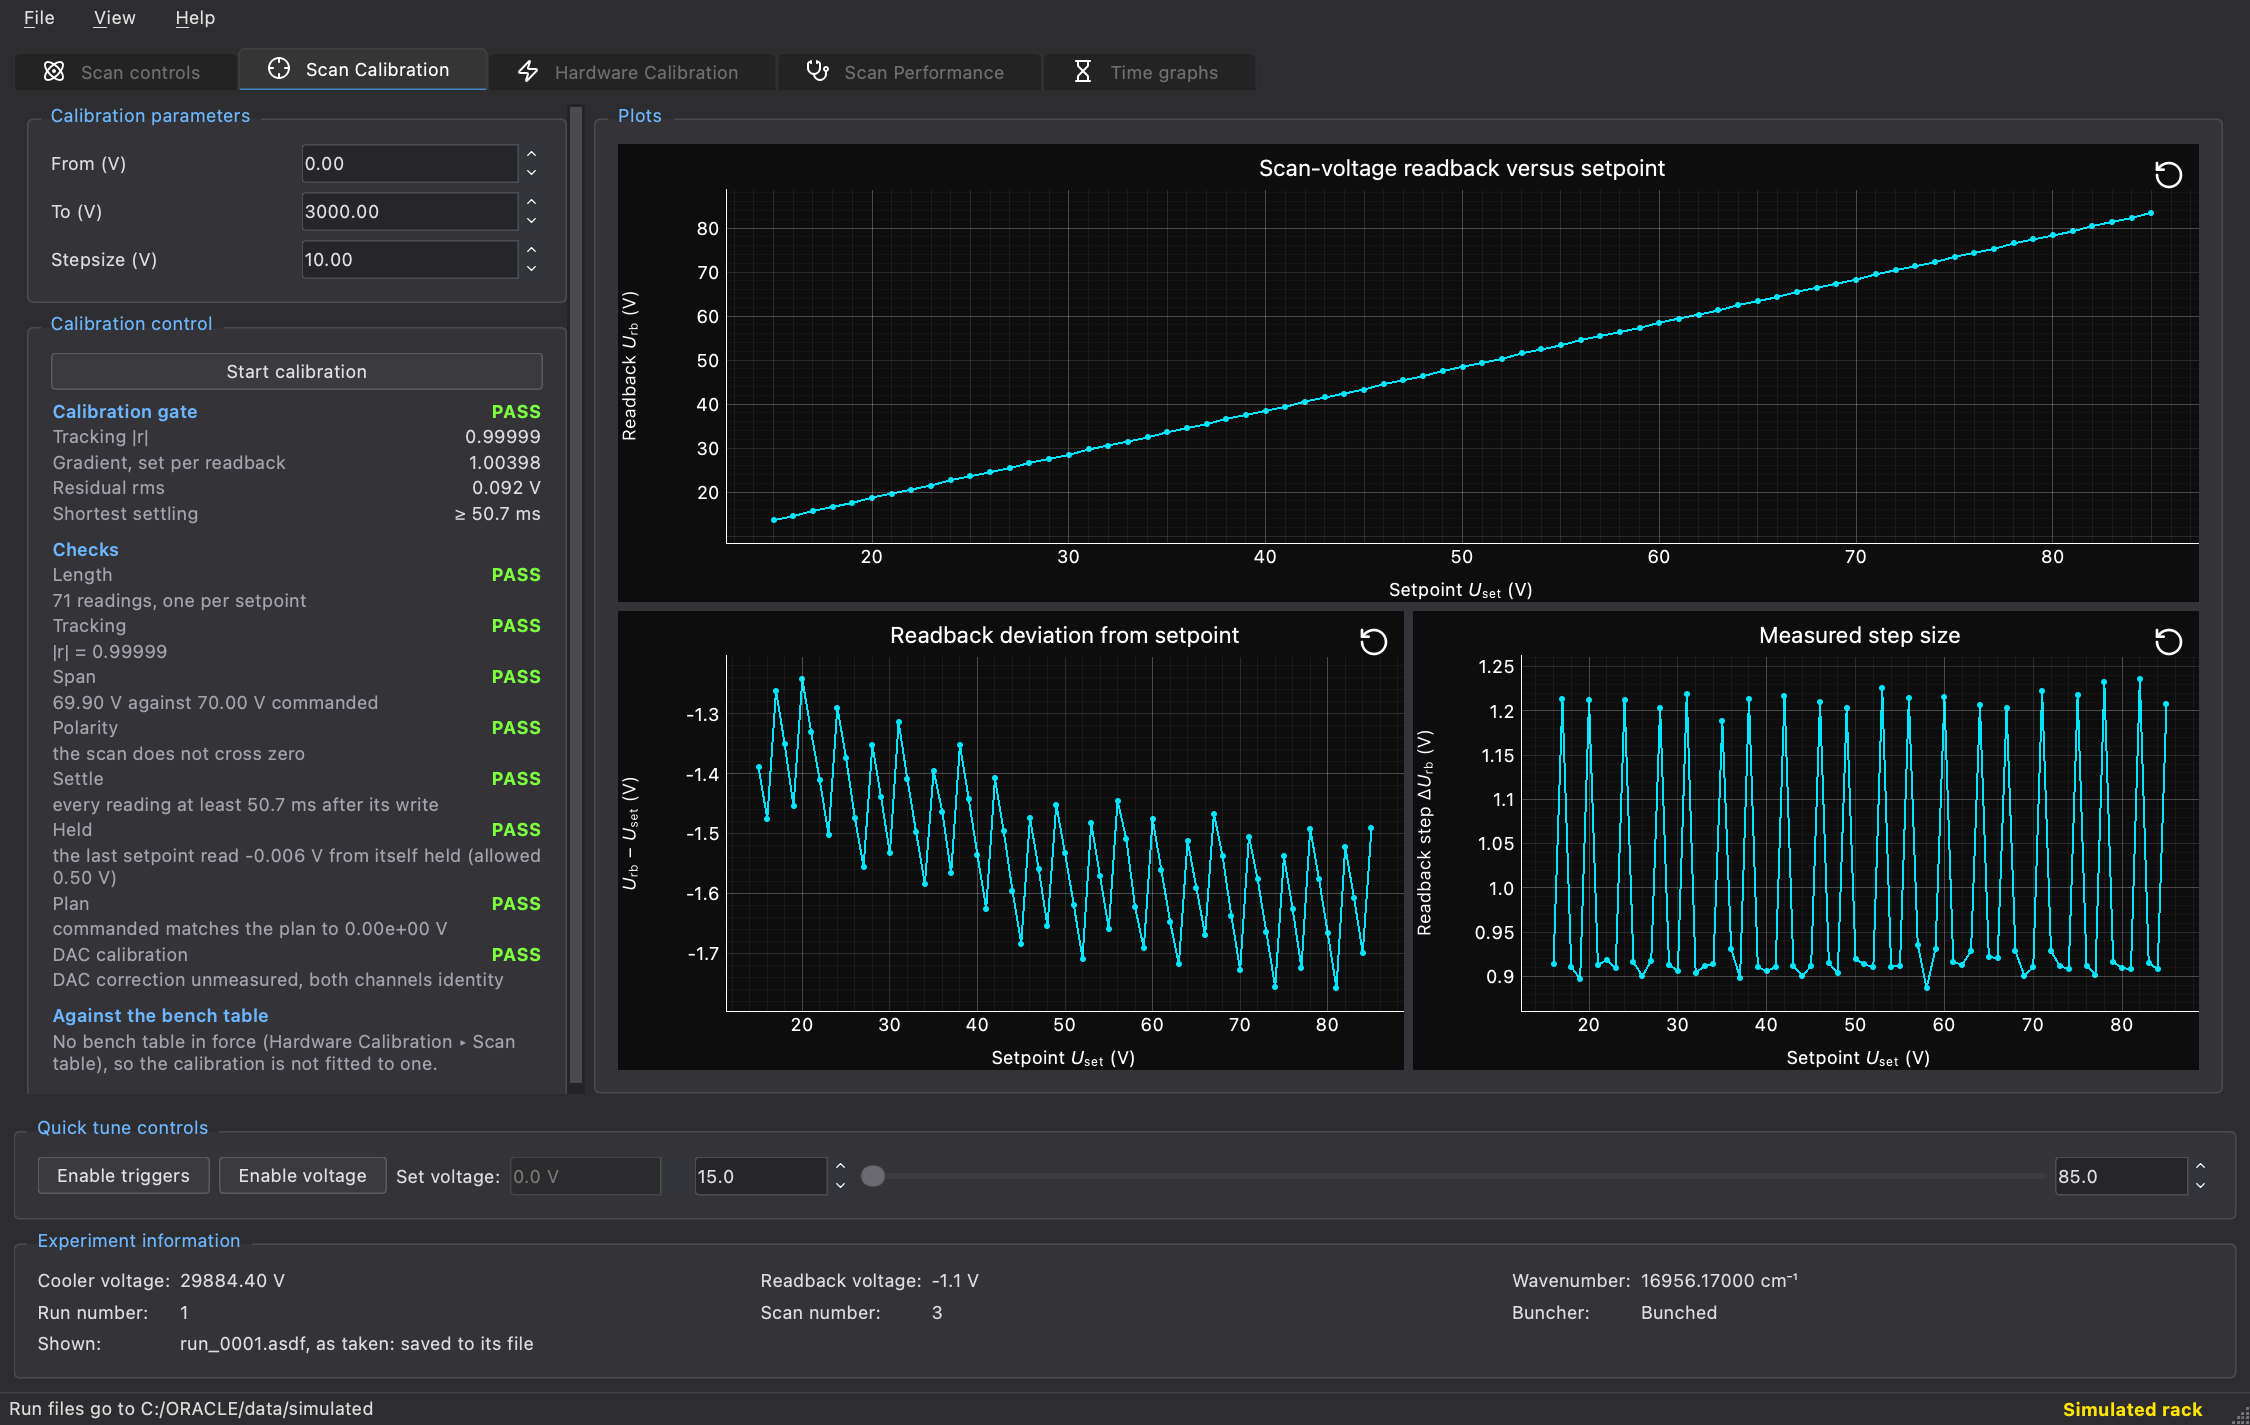
\includegraphics[width=\textwidth]{fig_calibration_tab}
    \caption{\app{Scan Calibration}: a run's calibration and the gate's report on it.}
    \label{fig:calibration}
\end{figure}

\section{Hardware Calibration}
\label{sec:hardware}

The bench calibration tool cls-cal~\cite{clscal} in \oracle{}: measurements of the rack
itself, one page each, laid out as the other tabs (parameters, buttons and result on the
left, plots on the right). Above the pages, \app{Ramp between points} sets the pace of
every unmeasured move, and \app{Line meter: Read (5 $\times$ NPLC 10)} reads the platform
precisely, to check the wiring and polarity against quick tune.

Every measurement drives the DAC by step and confirm, ramps back to 0\,V however it ends,
and writes its record under \code{<data>/hardware\_calibration/} as it goes, so a stopped
or failed one keeps what it took and is analysed as far as it went. On the rack each first
asks the operator to arm the high voltage, naming the most it will apply. \app{Open record...}
shows a record saved earlier, here or on another PC.

\subsection{Settle time}

Steps the platform out and back while the line meter samples on its own timer, and reports
each step's lag, settling and 10--90\,\% rise, overshoot and noise; optionally a \app{Drift
tail} at a long integration. \app{Use as scan settle model} puts the result in force for
scans; \app{Use recommended wait for linearity} sets the sweep's wait to three times the
slowest step (at least 0.2\,s).

\subsection{Linearity}

A count-based ladder up, down, up then down, or in random order (which separates drift from
shape), finer across 0\,V, with 0\,V read again every few rungs and several readings a point
with autozero. It reports gain and offset, residual, curvature, each converter's line and
where they meet 0\,V, hysteresis, the 0\,V drift and, from a dense sweep, each converter's
integral non-linearity. \app{Use as DAC correction} puts a correction in force for
\app{Valid for} days; production runs write uncorrected, since the bench table is applied
after collection, so a correction in force is warned of at every calibration.

\subsection{Cooler monitor}

Streams the cooler meter without gaps, at a short aperture (ripple) or an NPLC (drift), and
reports level, drift, noise by decade, the white-noise floor, the oscillations (mains
harmonics named, corrected for the meter's own attenuation) and the averaged spectrum.

\subsection{Scan table}
\label{sec:table}

The bench table gives the platform voltage each DAC code really gives; each run's
calibration is fitted to it (Section~\ref{sec:calibration}). On the bench tool's records,
the 25 October table predicts the next day's sweep to 11.6\,mV rms once $a + b\,T$ is
fitted.

\begin{description}
    \item[\app{Measure table}] sweeps \app{Span} $\pm$1\,kV (about 1.5\,h) or $\pm$3\,kV
        (about 5\,h, overnight) in 1\,V steps, 5 readings at NPLC 10 a point, 0\,V every 10
        points, \app{Order} up or random, at the Linearity page's settle time and watched
        there. The page warns while the 0\,V checks say the rack is still warming up. The
        sweep is made into a table when it completes.
    \item[\app{Resume...}] takes up a sweep that stopped, from its record, after its last
        0\,V check; the records make one table.
    \item[\app{Check table}] (start of a shift, after a power cycle) reads 250 points across
        the table's span in a few minutes and fits them to it: PASS at 15\,mV rms or less,
        else WARN, measure it again.
    \item[\app{Make from a linearity record...}] builds a table from any sweep with 0\,V
        checks. Tables are kept in \code{<data>/tables/}, named by date and ID (the hash of
        their contents), never overwritten.
    \item[\app{Use a table...}, \app{Compare with...}, \app{Use none}] put one in force, set
        another against it code by code, or use none.
\end{description}

The page shows each converter's shape about a straight line, the 0\,V level's drift and how
often 0\,V should be checked in a run (Figure~\ref{fig:table}). A table from another rack,
or one the settings name that is missing, is warned of at start-up, never refused.

\begin{figure}[ht]
    \centering
    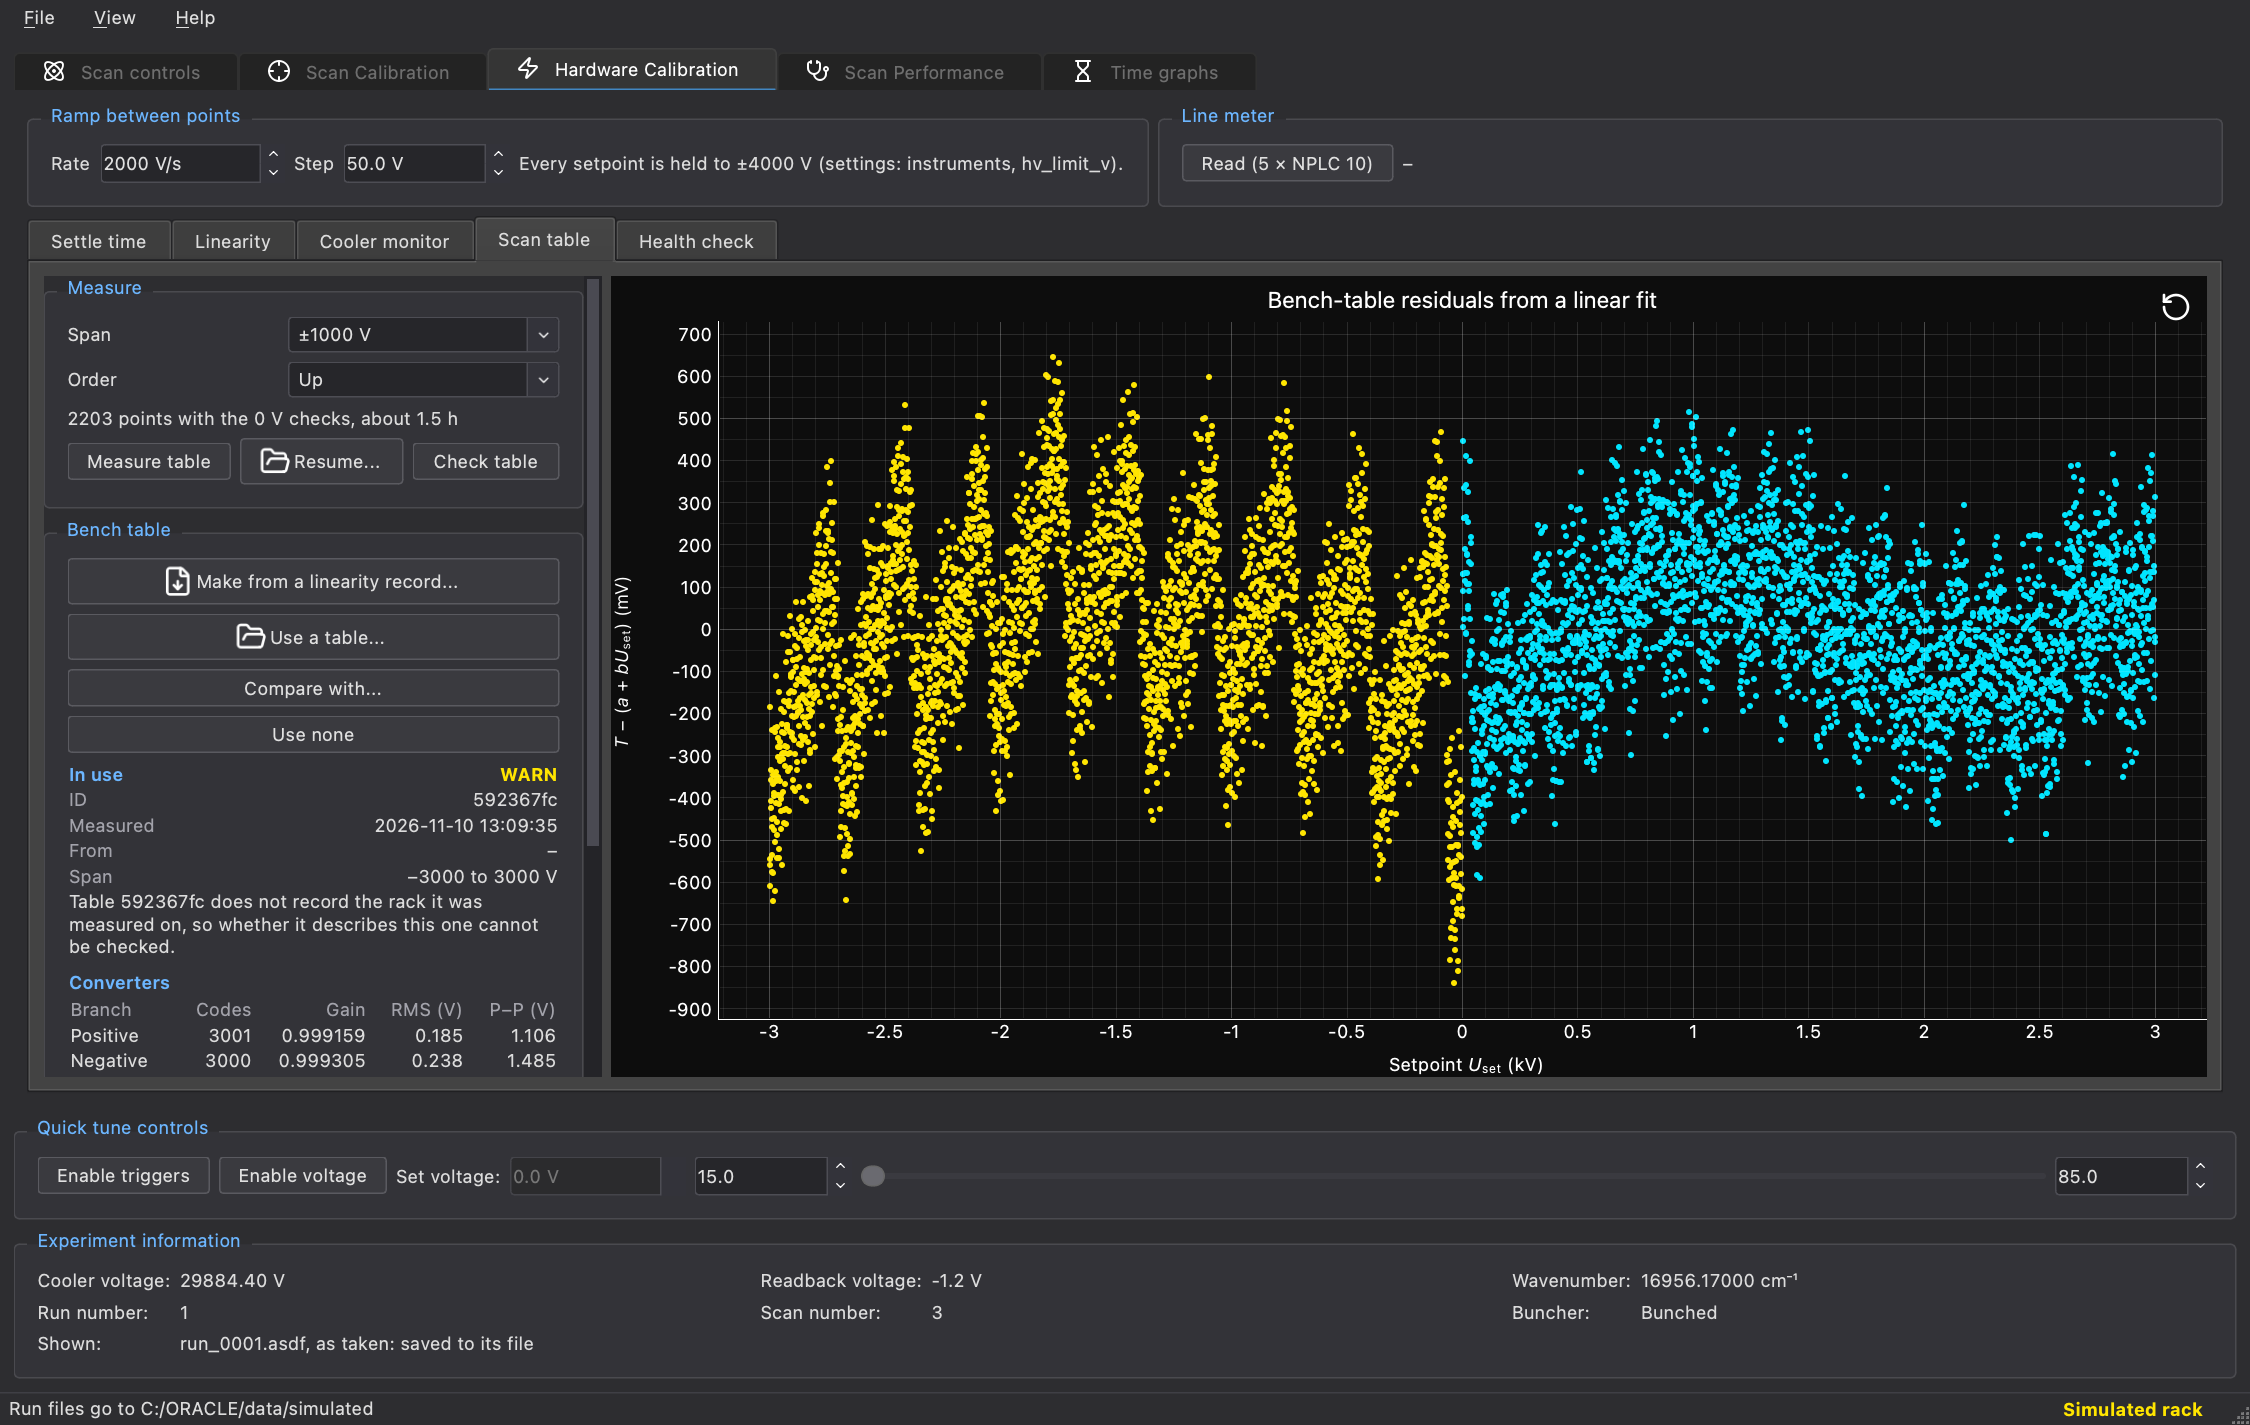
\includegraphics[width=\textwidth]{fig_hardware_table}
    \caption{The \app{Scan table} page with the 25 October 2026 bench table in force: each
        converter's residual from a straight line.}
    \label{fig:table}
\end{figure}

\subsection{Health check}

One report, at the start of a shift, on whether the rack is as it should be
(Figure~\ref{fig:health}). With \app{Check the bench table first} and a table in force it
runs the table check; then it reads the cooler for 10\,s (its 50\,Hz ripple), runs the Scan
tab's triggers for 10\,s counting each PMT (with the beam off, its dark counts) and the
triggers, and reads both meters' trigger sources. Each part is set against the last check:
WARN for ripple grown by half, a PMT silent or changed more than twice over, a trigger
miscounted or lost, or a meter on its trigger input. Every check is kept as
\code{hardware\_calibration/health\_<time>.yaml}; \app{Post to ELOG} posts it.

\begin{figure}[ht]
    \centering
    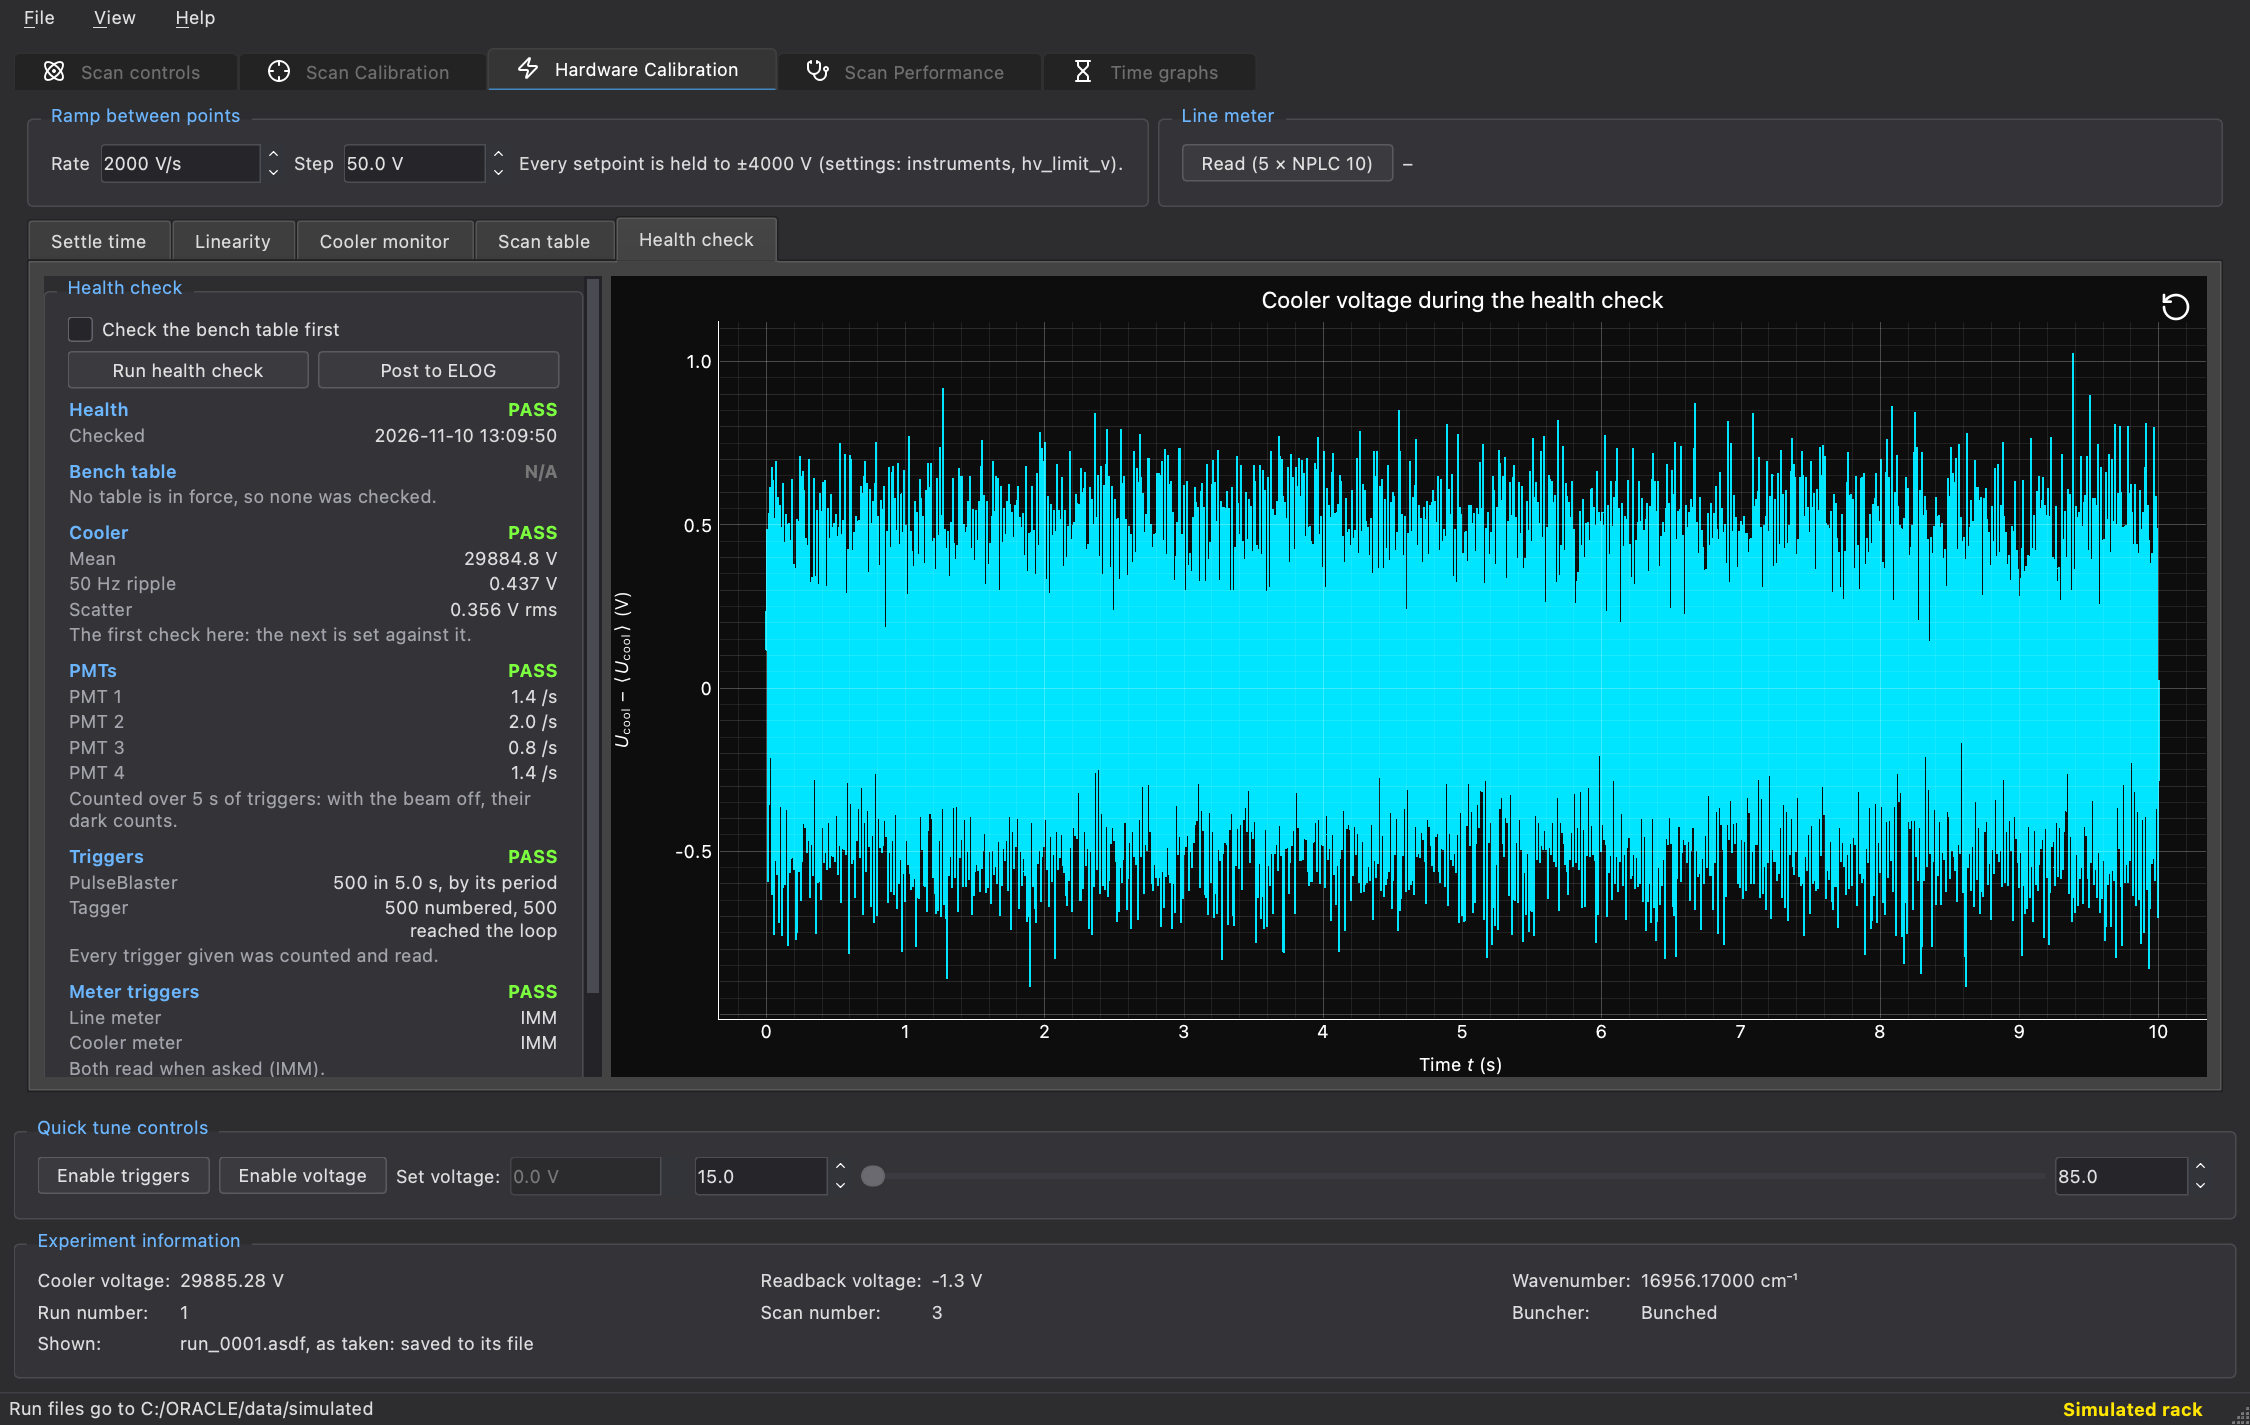
\includegraphics[width=\textwidth]{fig_health_check}
    \caption{A health check on the simulated rack, and the cooler it read.}
    \label{fig:health}
\end{figure}

\section{Scan Performance and Time graphs}
\label{sec:performance}

\subsection{Scan Performance}

How the rack's behaviour during a run shaped its spectrum (Figure~\ref{fig:performance}).
With \app{Analyse each run as it ends} ticked, each run is analysed as it closes; any other
is chosen under \app{Dataset} (the refresh button looks for new runs, the folder button
takes one from anywhere) and shown on every tab by \app{Show and analyse}.

Every check gives PASS, WARN, FAIL or N/A with the number it decided on; the
\app{Verdict} is the worst, with the line's width and what moved it. A deviation is flagged
only when it is both improbable under counting statistics and large enough to matter
against the line's width. Select a check to read what it found.

\begin{description}
    \item[Voltage scan.] Hits tagged with a voltage other than their bunch's; the
        calibration as \denis{} fits it, and against earlier runs calibrated the same way;
        the HV during the scan against its calibration.
    \item[Timing.] Whether the loop kept up with the triggers, stalls and pauses (a sleeping
        PC shows here), bunches taken before their step settled, missed triggers, the TOF
        peak against its gate.
    \item[Beam and spectrum.] Beam losses and stability, the line's position scan by scan
        against what the HV and laser monitors predict, the spectrum's shape, each channel.
    \item[Sources.] The cooler as the analysis takes it, a rolling mean over
        \code{cooler: rolling\_s} (15\,s), how far the readings scatter about it, and
        whether each hit's own reading is what its ions saw; the laser through the Doppler
        shift.
    \item[Detectors.] Each PMT's afterpulsing: its counts within \code{dead\_time\_us} of
        its own beyond what the other PMTs show, its scatter across scans against dead
        time, and a dead time suggested for \denis{}, never applied.
\end{description}

\app{Flagged for review} lists what deserves a look, with its reason; nothing is cut.
\app{Systematic inputs} gives each source of error as a width at the line, in scan volts
and MHz, marked measured, declared (in the settings) or not yet known; the Monte Carlo
that turns them into errors is \denis{}'s. A short block goes to the ELOG as each run is
analysed; \app{Post systematics to ELOG} posts the whole table. \app{Export report} writes
\code{run\_NNNN\_performance.yaml} and \code{run\_NNNN\_systematics.yaml} beside the run.

\begin{figure}[ht]
    \centering
    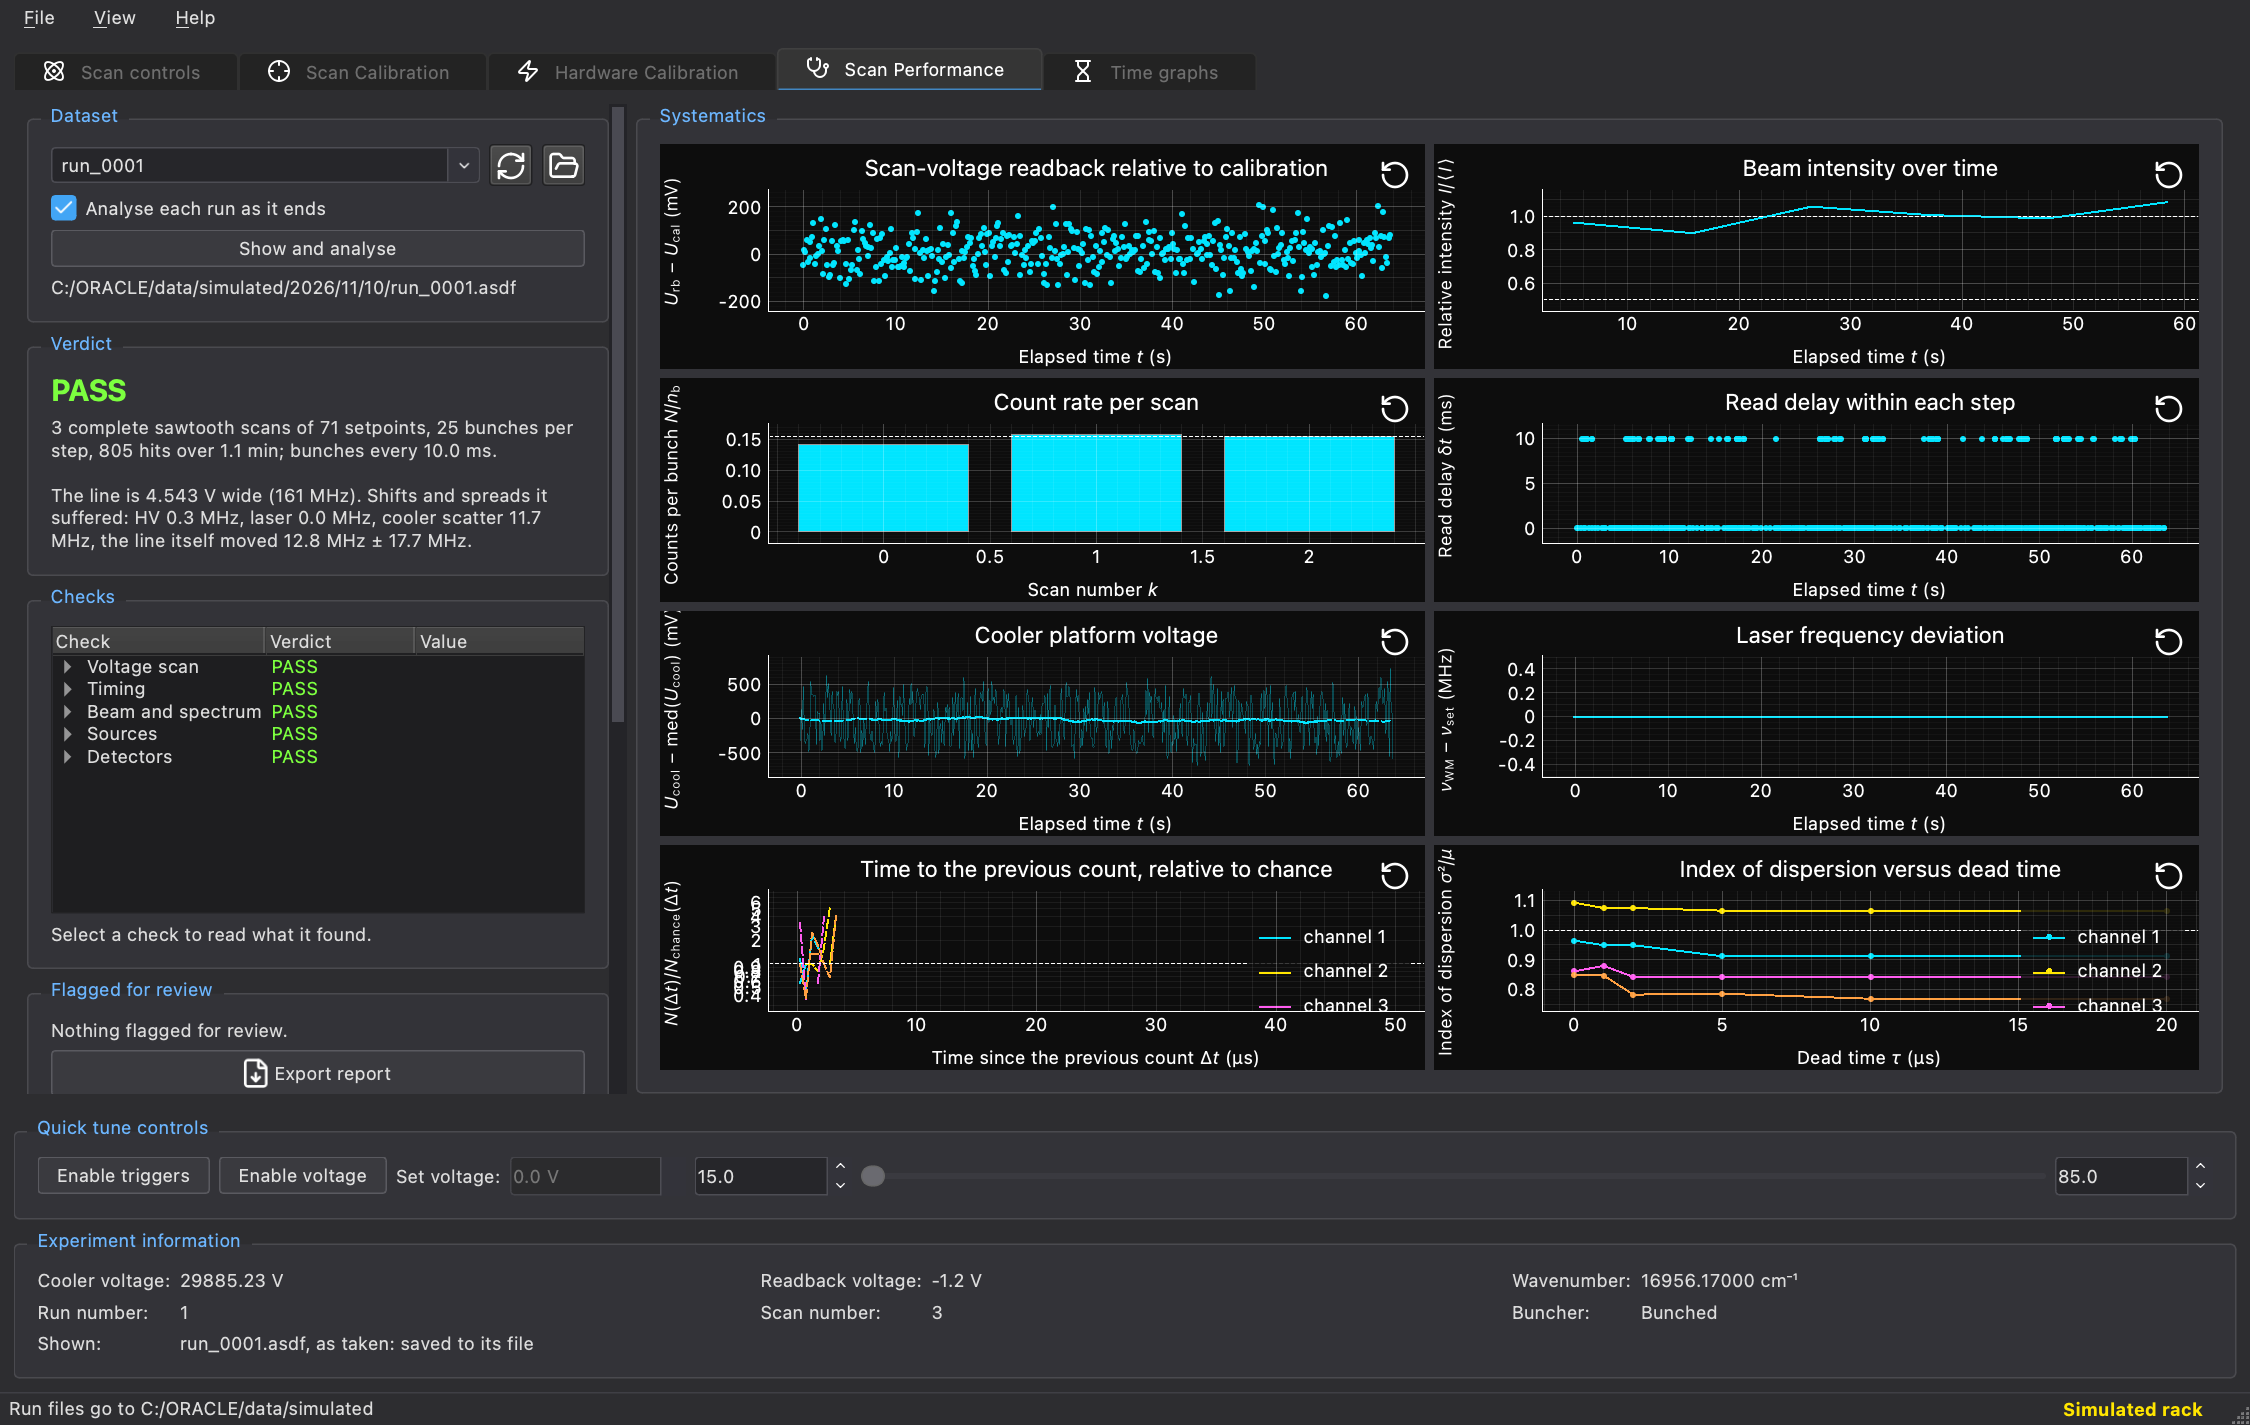
\includegraphics[width=\textwidth]{fig_performance_tab}
    \caption{\app{Scan Performance} for a simulated run: the verdict and checks, and a plot
        per systematic.}
    \label{fig:performance}
\end{figure}

\subsection{Time graphs}

Counts against time for the chosen channels, in bins of 100\,s down to 0.1\,s at the trigger
rate in force, to watch the beam. Below, each PMT's afterpulse ratio as data arrive: its
pairs within the dead time on itself over those on the others, 1 by chance, shown in the
warning colour above 2.

\section{Settings}
\label{sec:settings}

\code{settings/settings.yaml} holds what differs from the defaults in
\code{cls\_acquisition/settings.py}; it is written as settings are saved, and can be edited
while \oracle{} is closed. A file \oracle{} cannot read (a Windows folder in double quotes,
say) is refused at start-up with its line, never replaced by defaults.

\begin{center}
\small
\begin{tabularx}{\textwidth}{@{}lL@{}}
\toprule
Key & Meaning (default) \\
\midrule
\code{rack} & \code{simulated} or \code{hardware} \\
\code{data\_directory} & where runs go on the rack (\code{<app>/data}); a simulated rack writes to
    \code{<app>/data/simulated} \\
\code{experiment} & the experiment name, saved as it is edited \\
\code{elog} & \code{enabled}, \code{url}, \code{author} (disabled; never from a simulated rack) \\
\code{pvs} & EPICS names of the wavenumber, mass, mass setpoint and each input's PMT HV
    (\code{pmt\_hv\_1}--\code{4}) \\
\code{hardware} & what the rack cannot say: \code{scan\_divider} and \code{cooler\_divider}
    (\code{model}, \code{serial}, \code{ratio}, \code{ppm}; ratios 1000 and 10000) and the
    \code{amplifier}; recorded with every run \\
\code{instruments} & VISA resources of both meters, the MCC board (\code{dac\_board}), the
    tagger driver's folder and thresholds, \code{hv\_limit\_v} (4000, the most allowed) and
    \code{settle\_gate\_bit} (the MCC line gating the tagger; empty: not wired) \\
\code{dac\_correction} & a measured DAC correction (identity), written by \app{Use as DAC
    correction} \\
\code{scan\_table} & the ID of the bench table in force (none) \\
\code{settle\_model} & the scan's settling against jump size (none: SETTLE), written by
    \app{Use as scan settle model} \\
\code{calibration} & \code{nplc}: power line cycles a calibration reading integrates (1) \\
\code{cooler} & \code{rolling\_s}: the window of the cooler's rolling mean (15\,s) \\
\code{detectors} & \code{dead\_time\_us}: the dead time the PMTs are judged at (10\,\us) \\
\code{systematics} & \code{beam\_offset\_v} by region as \code{[offset, error]},
    \code{zero\_drift\_v} (0.030), \code{wavemeter\_mhz} (10) \\
\code{laser} & harmonic (4), geometry (anti-collinear) and charge (1) \\
\code{cooler\_pv} & publish the cooler as EPICS PVs (\code{FURIOS:Cooler:}; needs pcaspy) \\
\bottomrule
\end{tabularx}
\end{center}

Beside it, \code{inputs.yaml} keeps every input in the window, written half a second after
a change and whole, so a crash leaves the last complete set; delete it to start from the
defaults. \code{rack.yaml} keeps the last rack of each kind, so a change of hardware is
named at start-up.

\section{Data and records}
\label{sec:data}

\subsection{Run files}

Runs are written as the collinear DAQ wrote them, so cls\_tools and \denis{} read them
unchanged: \code{<data>/<year>/<month>/<day>/run\_NNNN.asdf}, ASDF standard
1.5.0~\cite{asdf}. The header holds the archive's sixteen keys, checked as it is written
(\code{CalSet} and \code{CalReadback} are the calibration), and the events follow as rows of

\begin{center}
\code{timestamp, voltage, bunch\_number, channel, time, cooler}
\end{center}

\noindent where \code{bunch\_number} counts the scan's bunches from 0, exactly
\code{BunchesPerChannel} a step, and \code{cooler} is the meter's reading in force for the
hit (times 10000 for the platform). A run's number is one more than the highest in the data
folder, so numbers survive a restart and a refused calibration leaves no gap.

One more header key, \code{ORACLE}, holds \oracle{}'s own record of the run; readers that
look keys up by name pass over it, and \menu{File > Open run...} restores the window from
it.

\begin{center}
\small
\begin{tabularx}{\textwidth}{@{}lL@{}}
\toprule
Key & Contents \\
\midrule
\code{Version}, \code{Commit} & \oracle{}'s version and git commit (\code{Hash}, \code{Dirty}) \\
\code{ScanType}, \code{Rounds}, \code{Queue} & the scan type, scans asked for, place in the queue \\
\code{Timing}, \code{View} & the trigger timing sent to the rack; the plots' view \\
\code{Calibration}, \code{CalibrationReadings} & the gate's verdicts and numbers; the
    readings' NPLC and the calibration's duration \\
\code{SettleModel}, \code{Laser}, \code{Channels} & the settle model, laser geometry and
    wired inputs \\
\code{CoolerRollingS}, \code{DeadTimeUs} & the cooler's rolling window; the PMTs' dead time \\
\code{Rack}, \code{RackIdentity} & simulated or hardware; the meters', DAC board's, tagger
    wrapper's and amplifier's identities \\
\code{Dividers} & both dividers as set; readers scale by these, never by today's settings \\
\code{DacCodes}, \code{DacCorrectionFull} & the converter and code each setpoint was
    written as; the DAC correction in full \\
\code{TaggerLevels} & each input's threshold \\
\code{ScanTable}, \code{TableFit} & the bench table in force; the calibration's fit to it \\
\code{InteractionRegion}, \code{ReferenceRun}, \code{PmtHv} & what the operator gave \\
\bottomrule
\end{tabularx}
\end{center}

\subsection{Files beside a run}

\begin{center}
\small
\begin{tabularx}{\textwidth}{@{}lL@{}}
\toprule
File & Contents \\
\midrule
\code{run\_NNNN\_monitor.csv} & the rack every 0.1\,s, written once a second: \code{time},
    \code{round}, \code{setpoint\_v}, \code{readback\_v}, \code{cooler\_v},
    \code{wavenumber\_cm1}, and the loop's \code{bunches}, \code{dropped}, \code{skipped} \\
\code{run\_NNNN\_performance.yaml} & the Scan Performance report: verdict, checks, flags,
    suggested dead times \\
\code{run\_NNNN\_systematics.yaml} & the systematic inputs \\
\bottomrule
\end{tabularx}
\end{center}

\subsection{Bench records and tables}

Hardware calibrations write CSV records under \code{<data>/hardware\_calibration/}:
\code{settle\_*}, \code{linearity\_*}, \code{cooler\_*} and their companions, each with its
settings as \code{\#} lines above the columns, rows flushed as taken, and its status and
results below; health checks as \code{health\_<time>.yaml}.

Bench tables, proposed as the format for cls\_tools, are kept as

\begin{center}
\code{<data>/tables/table\_<YYYYMMDD>\_<id8>.csv}
\end{center}

\noindent one row per converter and code,
\code{channel, code, setpoint\_v, volts, sigma\_v, readings}, where \code{channel} 0 drives
the positive branch, \code{volts} is the platform voltage relative to the 0\,V level, and
\code{\# key: value} lines (JSON values) above give its \code{id} (the SHA-256 of every
number), when and on which rack it was measured, its source record, the dividers, the 0\,V
drift and the recommended 0\,V check interval. A run's codes (\code{DacCodes}) and table
(\code{ScanTable}) let its calibration be fitted as $V = a + b\,T(\text{code})$. It reads
with

\begin{lstlisting}[language=Python]
pandas.read_csv(path, comment='#')
\end{lstlisting}


\appendix
\section{What ORACLE closes in the old DAQ}
\label{sec:design}

\begin{center}
\small
\begin{tabularx}{\textwidth}{@{}>{\raggedright\arraybackslash}p{0.38\textwidth}L@{}}
\toprule
Fault in the collinear DAQ & In \oracle{} \\
\midrule
D1, Mode A: two threads on one meter could leave a burst ungated & One owner thread per
    instrument, and VISA's exclusive lock between programs; every reading is taken on
    command, never on the meter's trigger input (PulseBlaster channel 17), which each mode
    reads back \\
D2, Mode B: setpoint $i$ read as reading $i + k$ & Step and confirm: no lag by construction,
    and the held check refuses one from any route \\
D3, Mode C: a fixed shape read as a seam at 0\,V & The platform runs on through 0\,V; the
    shape is each converter's gain and non-linearity, measured and fitted by the bench table \\
D4: the DC path recorded nothing & DC hits come through the tagger \\
D5: a read that timed out moved the scan on & A timed-out read is no bunch; a silent tagger
    is reported and the scan holds \\
Mode B's root: one bunch per tagger read & Each trigger is a bunch by the card's own number;
    a skipped number is a lost trigger, reported \\
D6: plans gained a point & Plans are counted, then laid down; never past the stop \\
D7: nothing inspected a calibration & The gate, before anything is written \\
D8, D9: two sessions on one instrument; dead code & One session per resource; not carried
    over \\
A dead acquisition process hung the window; a crashed window left the rack held & One reply
    per instruction, a dead process reported; the process watches its parent and leaves the
    platform at 0\,V \\
The tagger wrapper: inputs 3--4 on input 2's edge, rollover marks as hits, failed opens
    printed, empty triggers unmarked & The corrected wrapper (Section~\ref{sec:installation});
    a rack warning until it is built \\
Overload marks passed for voltages; meters left streaming by another program & Every
    reading checked; meters reset and identified on opening \\
The cooler's PV server opened the meter a second time & The PVs come from \oracle{}'s own
    readings \\
The bench tool lost an aborted sweep; its cooler blocks left gaps & Records written as they
    go; one stream \\
\bottomrule
\end{tabularx}
\end{center}

\section{Troubleshooting and known limits}
\label{sec:troubleshooting}

Every refusal is a sentence naming the fault and its numbers; the session log
(\menu{File > Open log folder}) keeps it with everything else.

\begin{center}
\small
\begin{tabularx}{\textwidth}{@{}>{\raggedright\arraybackslash}p{0.34\textwidth}L@{}}
\toprule
Seen & What to do \\
\midrule
\app{Rack warning} on the status bar & Read its tooltip: a fault \oracle{} cannot mend (the
    old tagger wrapper) or hardware changed since the last session (measure the settle
    model and the bench table again) \\
\app{Run rejected} after Start scan & The gate's failing check is named
    (Section~\ref{sec:calibration}); nothing was written. A \emph{held} or \emph{settle}
    refusal points at the meter or the settling; repeat, and measure the settle time \\
A timing refused before starting & Shorten the gate, release or delay, or lengthen the
    dwell, as the sentence says \\
No triggers reach the time tagger & Check the PulseBlaster, its cable to the tagger and the
    trigger level; the scan holds until triggers return \\
A meter shows NaN & It stopped answering its poll: check its USB and that no other program
    holds it \\
The settings are refused at start-up & Fix the named line (on Windows, use single quotes
    around a folder, or forward slashes) \\
The acquisition process stopped & The run is closed on what it recorded; restart \oracle{} \\
A queue stopped & Its row says why; fix it and start the queue again, which takes up at the
    first scan not done \\
\bottomrule
\end{tabularx}
\end{center}

\paragraph{Known limits.}
\begin{itemize}
    \item Nothing has yet run on the beamline; treat each hardware path as unverified until
        bench-tested on the rack PC.
    \item SETTLE comes from bench steps up to 2\,kV; the beamline's settle model should be
        measured across the jumps scans make, including the largest range join.
    \item The settle gate (an AND unit on PulseBlaster channel 18) is not wired: settling
        bunches are dropped in software, to within the USB latency.
    \item The DAC's codes are 0.305\,V apart, so a 1\,V step carries up to $\pm$0.15\,V of
        rounding that no correction removes; a step of a whole number of codes has none.
    \item The DAC correction drifts (offsets by up to 0.1\,V a day): keep its validity short.
    \item The live view keeps every hit of the run in memory, 11 bytes a hit: about 40\,MB
        an hour at 1000 hits a second.
\end{itemize}


\begin{thebibliography}{9}
\addcontentsline{toc}{section}{References}
\bibitem{clscal} A.~Raggio, \emph{cls-cal}: bench calibration tool for the IGISOL CLS rack
    (settle time, linearity, cooler monitor), 2026.
\bibitem{clstools} A.~Raggio, \emph{cls\_tools}: readers and sorting utilities for IGISOL
    CLS run files, \url{https://github.com/andry3vi/cls_tools}.
\bibitem{denis} A.~Kayaalp, \emph{DENIS}: Doppler Estimation and Numerical Inference for
    Spectroscopy, \url{https://github.com/ardakayaalp/DENIS}.
\bibitem{asdf} The ASDF standard, version 1.5.0, \url{https://asdf-standard.readthedocs.io}.
\end{thebibliography}

\end{document}
